\documentclass[10pt]{article}
\usepackage[margin=0.5in]{geometry}
\usepackage{amsmath, amssymb}
\usepackage{multicol}
\usepackage{graphicx}
\usepackage{circuitikz}


\setlength{\columnsep}{1.5cm}
\setlength{\voffset}{-0.25in}
\setlength{\parindent}{0in}


\title{
    \raggedright
    \large EECE 2150: Quiz 3 Notesheet \hfill Sean Balbale \hfill October 2024
    \vspace{-4em}
}
\date{}

\begin{document}
\maketitle

\begin{multicols}{2}
    
% SECTION 1: Logic Gates and Truth Tables
\section{Logic Gates and Truth Tables}

\subsection{AND Gate}
\textbf{Boolean Expression}: \( A \cdot B \) \\
\textbf{Truth Table}:
\[
\begin{array}{|c|c|c|}
\hline
A & B & A \text{ AND } B \\
\hline
0 & 0 & 0 \\\hline
0 & 1 & 0 \\\hline
1 & 0 & 0 \\\hline
1 & 1 & 1 \\\hline
\end{array}
\]

\subsection{OR Gate}
\textbf{Boolean Expression}: \( A + B \) \\
\textbf{Truth Table}:
\[
\begin{array}{|c|c|c|}
\hline
A & B & A \text{ OR } B \\
\hline
0 & 0 & 0 \\\hline
0 & 1 & 1 \\\hline
1 & 0 & 1 \\\hline
1 & 1 & 1 \\\hline
\end{array}
\]

\subsection{XOR Gate}
\textbf{Boolean Expression}: \( A \oplus B = \overline{A}B + A\overline{B}\) \\
\textbf{Truth Table}:
\[
\begin{array}{|c|c|c|}
\hline
A & B & A \text{ XOR } B \\
\hline
0 & 0 & 0 \\\hline
0 & 1 & 1 \\\hline
1 & 0 & 1 \\\hline
1 & 1 & 0 \\\hline
\end{array}
\]

\subsection{NAND Gate}
\textbf{Boolean Expression}: \( \overline{A \cdot B} \) \\
\textbf{Truth Table}:
\[
\begin{array}{|c|c|c|}
\hline
A & B & A \text{ NAND } B \\
\hline
0 & 0 & 1 \\\hline
0 & 1 & 1 \\\hline
1 & 0 & 1 \\\hline
1 & 1 & 0 \\\hline
\end{array}
\]

\subsection{NOR Gate}
\textbf{Boolean Expression}: \( \overline{A + B} \) \\
\textbf{Truth Table}:
\[
\begin{array}{|c|c|c|}
\hline
A & B & A \text{ NOR } B \\
\hline
0 & 0 & 1 \\\hline
0 & 1 & 0 \\\hline
1 & 0 & 0 \\\hline
1 & 1 & 0 \\\hline
\end{array}
\]

\subsection{XNOR Gate}
\textbf{Boolean Expression}: \( A \odot B = AB + \overline{AB} \) \\
\textbf{Truth Table}:
\[
\begin{array}{|c|c|c|}
\hline
A & B & A \text{ XNOR } B \\
\hline
0 & 0 & 1 \\\hline
0 & 1 & 0 \\\hline
1 & 0 & 0 \\\hline
1 & 1 & 1 \\\hline
\end{array}
\]

\subsection{NOT Gate}
\textbf{Boolean Expression}: \( \overline{A} \) \\
\textbf{Truth Table}:
\[
\begin{array}{|c|c|}
\hline
A & NOT A \\
\hline
0 & 1 \\\hline
1 & 0 \\\hline
\end{array}
\]
--- % New Section Divider
\section{NAND Gate Equivilance}
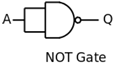
\includegraphics[width=0.2\textwidth]{NotGateFromNAND.png}
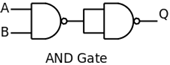
\includegraphics[width=0.2\textwidth]{AndGateFromNAND.png}\\
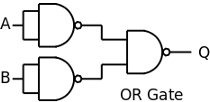
\includegraphics[width=0.2\textwidth]{OrGateFromNAND.png}\\
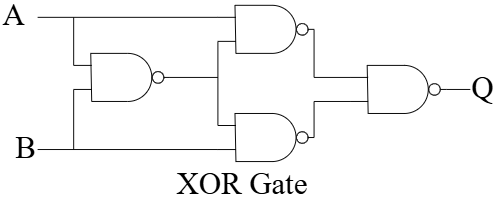
\includegraphics[width=0.4\textwidth]{XorGateFromNAND.png}\\
% 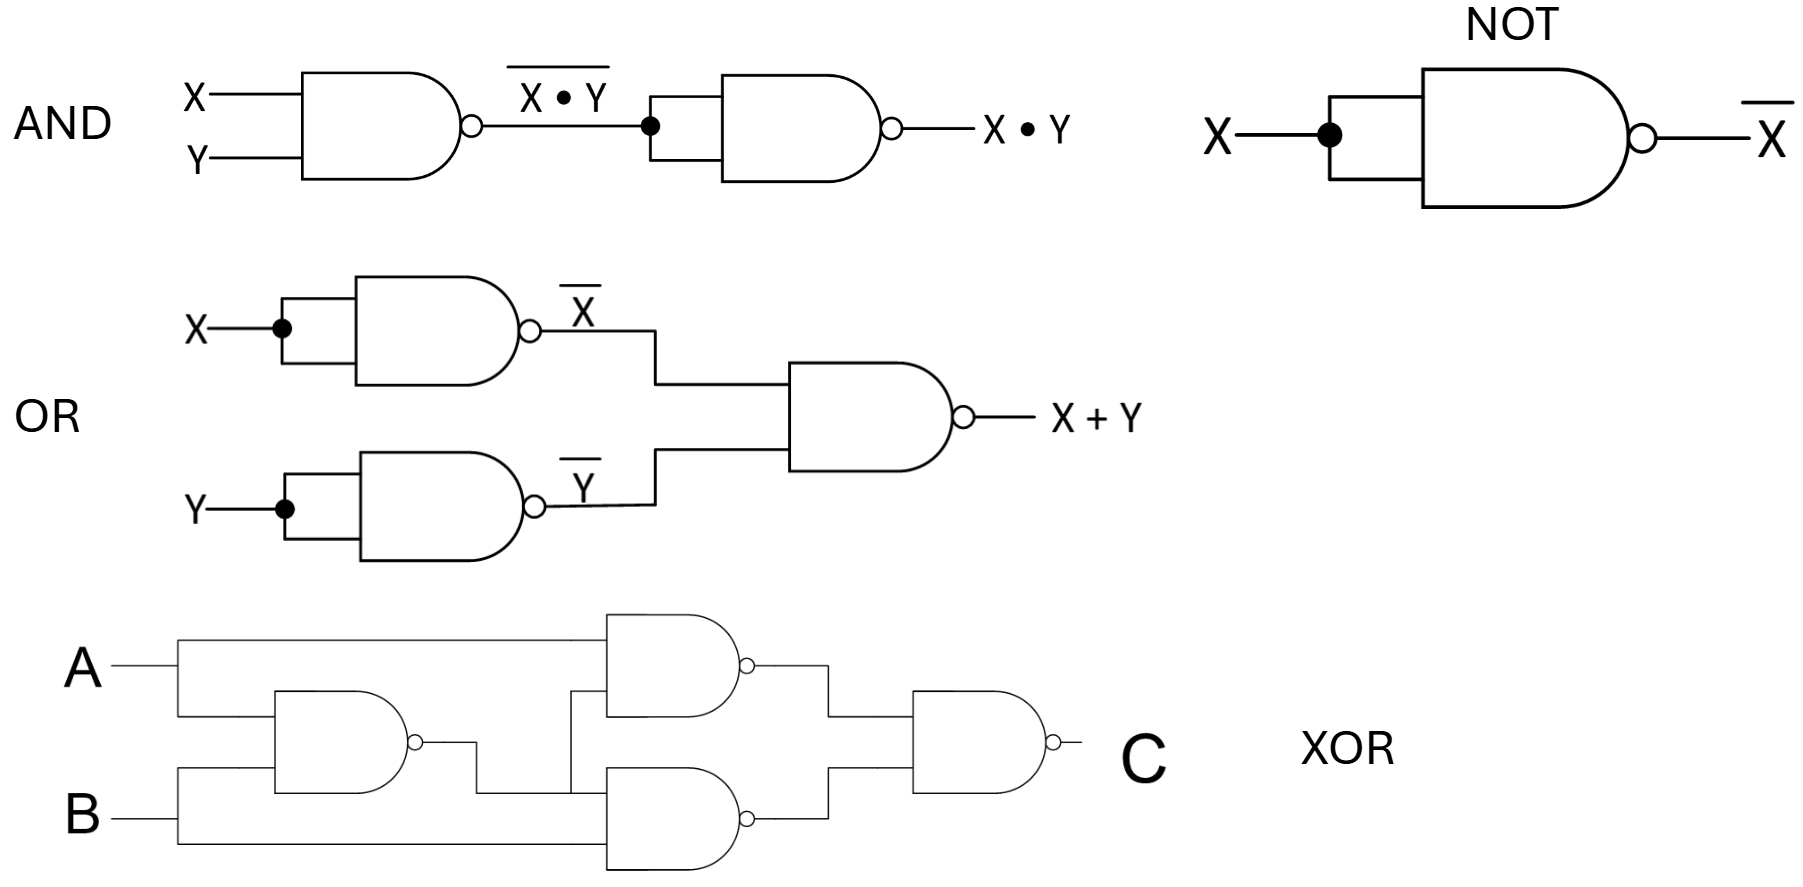
\includegraphics[width=0.4\textwidth]{NANDEquivilance.png}
--- % New Section Divider

% SECTION 4: Karnaugh Maps (K-Maps)
\section{Karnaugh Maps (K-Maps)}

Used to simplify Boolean expressions:
\begin{itemize}\itemsep0pt
    \item Group 1s in powers of 2 (1, 2, 4, 8...).
    \item Simplify terms by reducing variables.
\end{itemize}

\subsection{Example 4-Variable K-Map}
\[
\begin{array}{|c|c|c|c|c|}
\hline
AB \backslash CD & 00 & 01 & 11 & 10 \\
\hline
00 & X & 0 & 1 & 1 \\
\hline
01 & 1 & 1 & X & 0 \\
\hline
11 & 1 & 1 & X & 0 \\
\hline
10 & 0 & 0 & X & 1 \\
\hline
\end{array}
\]
\textit{This example shows a 4-variable K-Map with values for each combination of inputs (A, B, C, D). Group 1s in powers of 2 to simplify.}\\
$Y = \overline{A}C + A\overline{C} = A \oplus C$\\
--- % New Section Divider

% SECTION 2: Two's Complement
\section{Two's Complement}
\textbf{Two's Complement Conversion}:
\begin{enumerate}\itemsep0pt
    \item Invert all bits.
    \item Add 1 to the least significant bit (LSB).
\end{enumerate}
\textit{Example}: Convert \(5\) to binary and find \(-5\):
\[
5_{10} \rightarrow 0101 \rightarrow \text{Invert: } 1010 \rightarrow \text{Add 1: } 1011 \rightarrow -5
\]

\textbf{Overflow Detection}: This happens when a number larger than the maximum 
allowed number of bits occurs. When adding two numbers of the same sign, if the result’s sign differs from the operands, an overflow occurred.
\\
\textbf{Caryout Detection}: When the result has a one in the most significant bit + 1 position.

--- % New Section Divider

% SECTION 3: Multiplexers, Shifters, and Steady State Machines
\section{Multiplexers, Shifters, and Steady State Machines}

\subsection{Multiplexer (MUX)}
% A 2-to-1 MUX selects between inputs \( A \) and \( B \) based on \( S \):
% \[
% Y = A \cdot \overline{S} + B \cdot S
% \]
\subsubsection{2:1 Multiplexer}
\begin{itemize}
    \item \textbf{Description}: A 2:1 multiplexer has two inputs (\( A \) and \( B \)), one output (\( Y \)), and one select line (\( S \)).
    \item \textbf{Functionality}: The select line \( S \) determines which input is connected to the output \( Y \):
    \[
    Y = S' \cdot A + S \cdot B
    \]
    
    \item \textbf{Application}: Basic signal selection in low-complexity circuits.
\end{itemize}

\subsubsection{4:1 Multiplexer}
\begin{itemize}
    \item \textbf{Description}: A 4:1 multiplexer has four inputs (\( A, B, C, D \)), one output (\( Y \)), and two select lines (\( S_0 \) and \( S_1 \)).
    \item \textbf{Functionality}: The select lines \( S_0 \) and \( S_1 \) determine which input is routed to the output \( Y \):
    \[
    Y = S_1'S_0' \cdot A + S_1'S_0 \cdot B + S_1S_0' \cdot C + S_1S_0 \cdot D
    \]
    
    \item \textbf{Application}: Used for selecting one of multiple signals in data routing and control systems.
\end{itemize}

\subsection{Shifters}
Logical, Arithmetic, and Circular Shifters:
\begin{itemize}\itemsep0pt
    \item Logical Shifter: Moves all bits left or right by adding zero.
    \item Arithmetic Shifter: Left, same as logical, Right, skips most significant bit.
    \item Circular Shifter: Rotates bits.
\end{itemize}
% 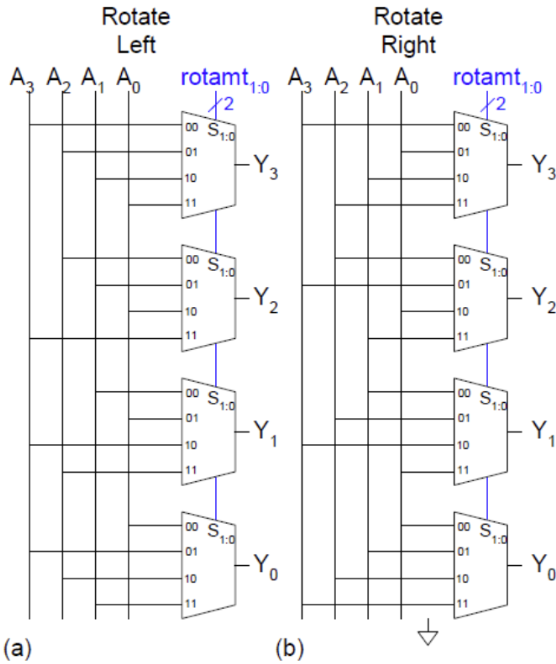
\includegraphics[width=0.4\textwidth]{Left and Right Rotators.png}

\subsection{Steady State Machines}
\textbf{Moore Machine}: Output depends on current state only. \\
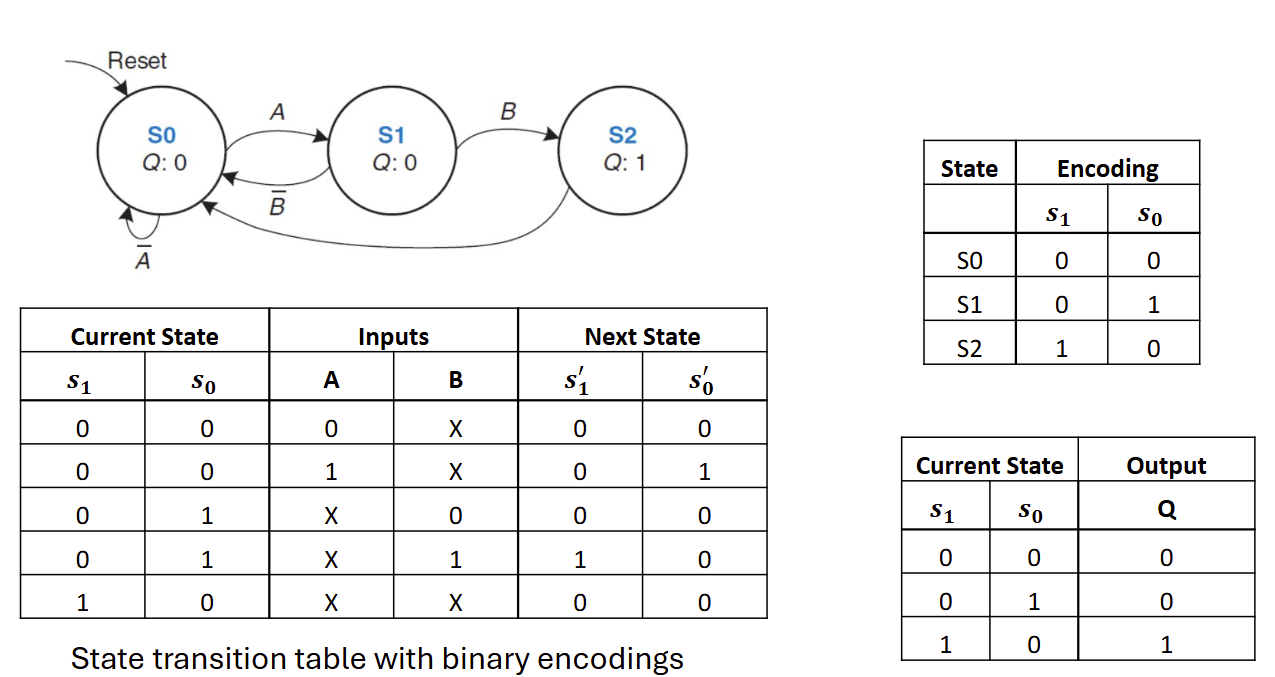
\includegraphics[width=0.4\textwidth]{moore machine example.png}

--- % New Section Divide

% SECTION 5: D Latch and Flip-Flops
\section{D Latch vs. D Flip-Flop}
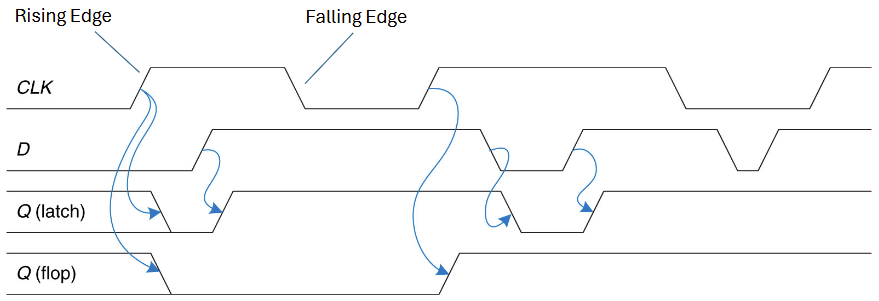
\includegraphics[width=0.4\textwidth]{D Latch vs Flip Flop.png}
\subsection{D Latch (Level-Triggered)}
\begin{itemize}
    \item \textbf{Functionality}: The D latch passes the input \( D \) to the output \( Q \) when the Enable signal (often denoted as \( E \) or \text{EN}) is active (high, or logic 1). When the enable is low (0), the output \( Q \) holds its previous value, effectively "latching" onto the last state.
    \item \textbf{Level-Triggered}: A D latch is \textbf{level-triggered}, meaning it responds to the level (high or low) of the enable signal. As long as the enable signal is high, changes at \( D \) will pass directly to \( Q \).
\end{itemize}

\subsection{D Flip-Flop (Edge-Triggered)}
\begin{itemize}
    \item \textbf{Functionality}: A D flip-flop captures the value at input \( D \) only at the moment of a clock edge (typically the rising or falling edge of the clock signal). The value of \( Q \) is updated only on the clock edge and then remains constant until the next clock edge.
    \item \textbf{Edge-Triggered}: Unlike the latch, the D flip-flop is \textbf{edge-triggered}, meaning it only updates \( Q \) on a specific transition of the clock signal (either rising or falling edge). This characteristic makes it useful in synchronous circuits.
\end{itemize}

\end{multicols}
\end{document}




